\documentclass[aspectratio=149]{beamer}
\usepackage[utf8]{inputenc}

\usepackage[utf8]{inputenc}
\usepackage[T1]{fontenc}

\usepackage[english]{babel}
\usepackage{amsmath}
\usepackage{cleveref}
\usepackage{amssymb}
\usepackage{mathtools}

%%Numbers, expectation
\newcommand{\N}{\mathbb{N}}
\newcommand{\E}{\mathbb{E}}
\renewcommand{\P}{\mathbb{P}}
\newcommand{\Var}{\mathbb{V}}
\newcommand{\R}{\mathbb{R}}
\newcommand{\D}{\mathcal{D}}
\newcommand{\B}{\mathcal{B}}
\newcommand{\Dh}{\D_h}
\renewcommand{\phi}{\varphi}
\newcommand*\diff{\mathop{}\!\mathrm{d}} % integral

%% mathoperator
\DeclareMathOperator*{\argmax}{arg\,max}
\DeclareMathOperator*{\argmin}{arg\,min}
\DeclareMathOperator*{\dom}{dom}
\DeclareMathOperator*{\sign}{sign}
\DeclareMathOperator*{\diag}{diag}

\DeclareMathOperator*{\Cov}{Cov}
\DeclareMathOperator*{\Cor}{Corr}
\DeclareMathOperator*{\Id}{Id}

%proximal operator
\newcommand{\prox}[3][]{\operatorname{prox}^{#1}_{#2}\left(#3 \right)}

\usepackage{xcolor}

%% sort citations by increasing number
\usepackage[sort,nocompress]{cite}

\usepackage{graphicx}% http://ctan.org/pkg/graphicx
\graphicspath{{../figures/}{../../figures}{../../memes}} %Setting the graphicspath
\usepackage{caption,subcaption}

\usepackage{tikz}
\usepackage{pgfplots}
\usetikzlibrary{backgrounds}
\usetikzlibrary{intersections}
\usepgfplotslibrary{fillbetween}

% \usepackage[right]{showlabels}


%%
\theoremstyle{plain}
\newtheorem{prop}{Proposition}[section]
\newtheorem{algo}{Algorithm}[section]
\newtheorem{assumption}{Assumption}
\theoremstyle{remark}
\newtheorem{remark}{Remark}[section]

% cref
\crefname{assumption}{Assumption}{Assumptions}
\crefname{equation}{}{}

\usepackage{autonum}

\usepackage{bm} %% bold math symbols

\usepackage{bbm} %% for \mathbbm{1}


% algorithmic environment
\usepackage{algorithm}
\usepackage[noend]{algpseudocode}

% for some reason this was required on one void linux installation (but not the other)
\usepackage{sansmathaccent}
\pdfmapfile{+sansmathaccent.map}

\author{Axel Böhm}

% shows which section we're in
\usetheme{Darmstadt}

% page number
\setbeamertemplate{footline}[frame number]
\setbeamercolor{page number in head/foot}{fg=gray}


% display things like onslide or visible already before but grayed out
\setbeamercovered{transparent}

% set the itemize item symbol as a diamond
\setbeamertemplate{itemize item}{$\diamond$}
% set the itemize subitem symbol as a triangle
\setbeamertemplate{itemize subitem}{$\blacktriangleright$}

% set the enumerate item symbol as a roman numbers
\setbeamertemplate{enumerate item}{(\roman{enumi})}


\author{Axel Böhm}

% shows which section we're in
\usetheme{Darmstadt}

% page number
\setbeamertemplate{footline}[frame number]
\setbeamercolor{page number in head/foot}{fg=gray}


% display things like onslide or visible already before but grayed out
\setbeamercovered{transparent}

% set the itemize item symbol as a diamond
\setbeamertemplate{itemize item}{$\diamond$}
% set the itemize subitem symbol as a triangle
\setbeamertemplate{itemize subitem}{$\blacktriangleright$}

% set the enumerate item symbol as a roman numbers
\setbeamertemplate{enumerate item}{(\roman{enumi})}


\newcounter{sauvegardeenumi}
\newcommand{\asuivre}{\setcounter{sauvegardeenumi}{\theenumi}}
\newcommand{\suite}{\setcounter{enumi}{\thesauvegardeenumi}}

\title{Nonconvex Optimization}
\date{\today}

\begin{document}
\maketitle
\frame{\tableofcontents}

\section{Introduction}

\begin{frame}
  \frametitle{Gradient Descent in the nonconvex world}

  may get stuck in a \textbf{\textcolor{blue}{local}} minimum and miss the global minimum

  \begin{figure}[ht]
    \centering
    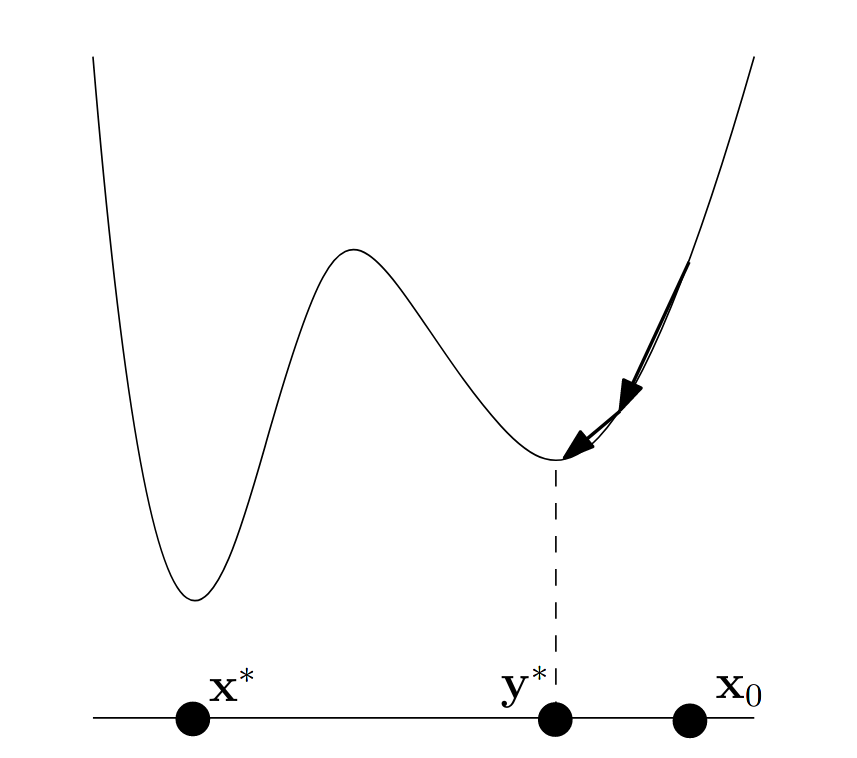
\includegraphics[height=0.8\textheight,keepaspectratio]{nonconvex.png}
  \end{figure}
\end{frame}


\begin{frame}
  \frametitle{Gradient Descent in the nonconvex world II}
  Even if there is a unique \textcolor{blue}{local} minimum (equal to the global minimum), we
  \begin{itemize}
    \item  may get stuck in a saddle point;
    \item run off to infinity;
    \item possibly encounter other bad behaviors.
  \end{itemize}
  \begin{figure}[ht]
    \centering
    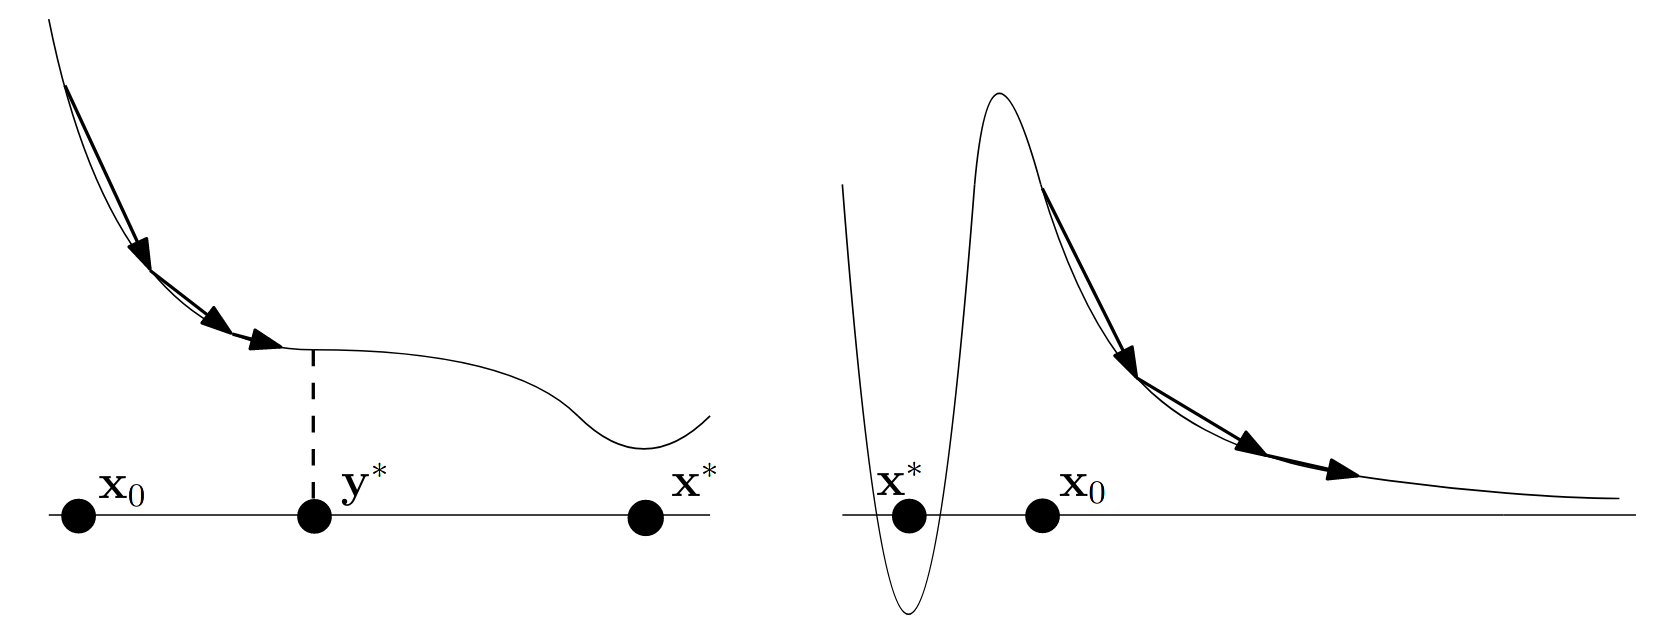
\includegraphics[width=\textwidth,height=\textheight,keepaspectratio]{nonconvex2}
  \end{figure}
\end{frame}


% \begin{frame}
%   \frametitle{Gradient Descent in the nonconvex world III}
%   \begin{itemize}
%     \item Often, we observe good behavior in practice.
%     \item Theoretical explanations many times missing.
%     \item This lecture: under favorable conditions, we sometimes can say something useful about
%   the behavior of gradient descent, even on nonconvex functions
%   \end{itemize}
% \end{frame}

\begin{frame}
  \frametitle{Smooth (but not necessarily convex) functions}
  \textbf{Recall}: A differentiable $f : \R^d \to \R$ is $L$-smooth over a convex set $X$ if
  \begin{equation}
    f(y) \le f(x) + \langle \nabla f(x), y- x \rangle + \frac{L}{2} \Vert y-x \Vert^2, \quad \forall x,y \in X.
  \end{equation}
  \begin{figure}[ht]
    \centering
    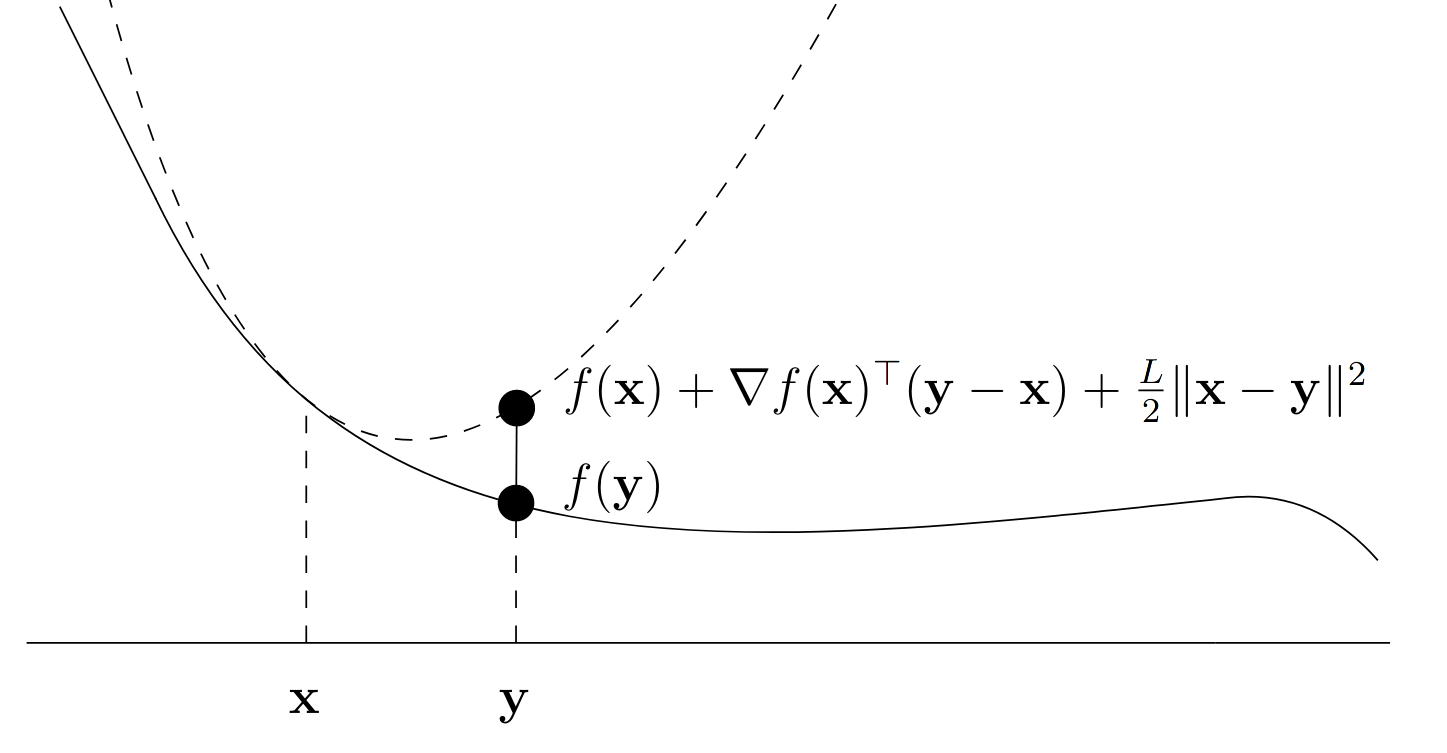
\includegraphics[height=0.65\textheight,keepaspectratio]{smoothness_no_convex}
  \end{figure}
\end{frame}


\begin{frame}
  \frametitle{Bounded Hessians $\Rightarrow$ smooth}
  \begin{lemma}%
    Let $f: \R^d \to \R$ be twice differentiable and
    \begin{equation}
      \Vert \nabla^2 f(x) \Vert \le L
    \end{equation}
    where $\Vert \cdot \Vert$ is spectral norm. Then $f$ is $L$-smooth
  \end{lemma}

  Examples:
  \begin{itemize}
    \item all quadratic functions $f(x)= x^T Ax + b^T x + c$
    \item $f(x) = \sin (x)$ (many global minima)
  \end{itemize}
\end{frame}


\begin{frame}
  \frametitle{Gradient descent on smooth functions}
  Will prove: $\Vert \nabla f(x_k) \Vert^2 \to 0$ for $k\to \infty$ \ldots \\
  \ldots at the same rate as $f(x_k) -f(x^*)$ →0 in the convex case.
  \begin{itemize}
    \item $f(x_k) -f(x^*)$ itself may not converge to 0 in the nonconvex case:
  \end{itemize}
  \begin{figure}[ht]
    \centering
    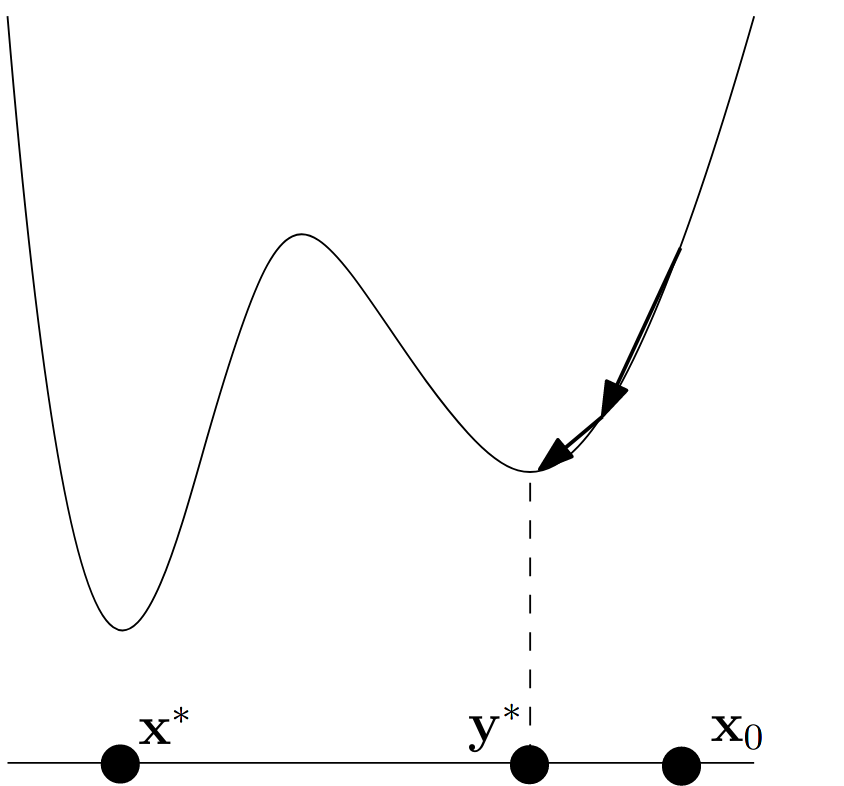
\includegraphics[height=0.7\textheight,keepaspectratio]{nonconvex_func}
    \caption{\label{fig:label} }
  \end{figure}
\end{frame}


\begin{frame}
  \frametitle{What does $\Vert \nabla f(x_k) \Vert^2\to 0$ mean?}

  \begin{itemize}
    \item May or \textcolor{blue}{may not} mean convergence to a critical point $\nabla f(y^*) =0$
    \item critical point might not be even local minimum
  \end{itemize}

  \begin{figure}[ht]
    \centering
    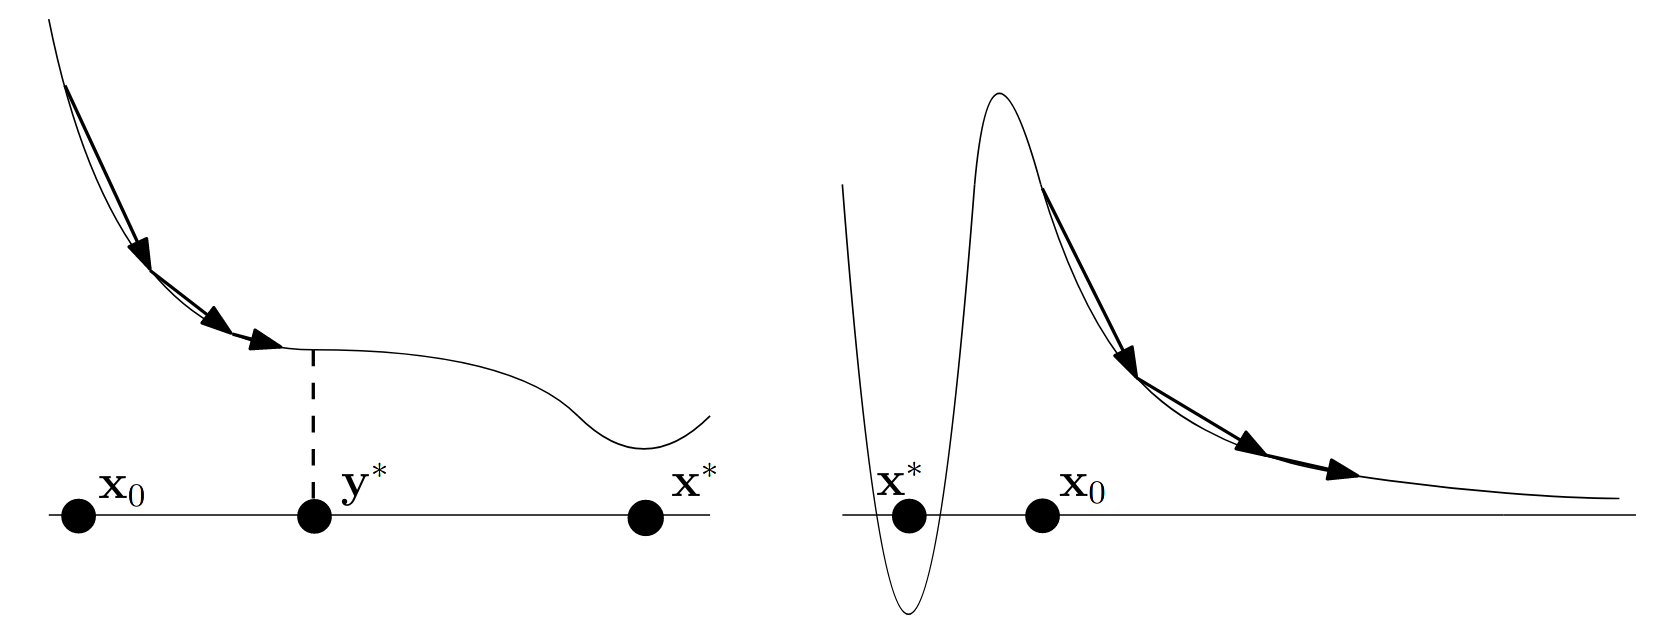
\includegraphics[width=\textwidth,height=\textheight,keepaspectratio]{nonconvex2}
    \caption{\label{fig:label} }
  \end{figure}
\end{frame}


\begin{frame}
  \frametitle{Gradient descent on smooth (not necessarily convex) functions}

  \begin{theorem}
    Let $f : \R^d \to \R$ be $L$-smooth with a global minimum $x^*$. \\
    Choosing stepsize $\alpha := \frac{1}{L}$ gradient descent yields
    \begin{equation}
      \frac{1}{K} \sum_{k=0}^{K-1} \Vert \nabla f(x_k) \Vert^2 \le \frac{2L}{K} \big(f(x_0) - f(x^*)\big).
    \end{equation}
  \end{theorem}
  In particular, same bound hold for ``best'' iterate
  \begin{equation}
    \min_{0\le k \le K-1} \Vert \nabla f(x_k) \Vert^2 \le \frac{2L}{K} \big(f(x_0)-f(x^*)\big)
  \end{equation}
  and
  \begin{equation}
    \lim_{k \to \infty} \Vert \nabla f(x_k) \Vert^2 = 0.
  \end{equation}
\end{frame}


\begin{frame}
  \frametitle{Gradient descent on smooth  functions II: Proof}

  Smoothness gives:
  \begin{equation}
    f(y) \le f(x) + \langle \nabla f(x), y- x \rangle + \frac{L}{2} \Vert y-x \Vert^2.
  \end{equation}
  Use $y=x_{k+1}$ and $x=x_k$
  \begin{equation}
    f(x_{k+1}) \le f(x_k) + \langle \nabla f(x_k), - \nabla \alpha f(x_k) \rangle + \frac{L \alpha^2}{2} \Vert \nabla f(x_k) \Vert^2
  \end{equation}
  to obtain \textcolor{blue}{sufficient decrease:}
  \begin{equation}
    f(x_{k+1}) \le f(x_k) - \frac{1}{2L} \Vert \nabla f(x_k) \Vert^2.
  \end{equation}
\end{frame}


\begin{frame}
  \frametitle{Proof II}
  \textcolor{blue}{sufficient decrease:}
  \begin{equation}
    f(x_{k+1}) \le f(x_k) - \frac{1}{2L} \Vert \nabla f(x_k) \Vert^2.
  \end{equation}
  Sum up from $k=0, 1, \dots, K-1$ to get
  \begin{equation}
      \frac{1}{2L}\sum_{k=0}^{K-1} \Vert \nabla f(x_k) \Vert^2 \le f(x_0) - f(x_{k}) \le f(x_0) - f(x^*).
  \end{equation}
  Multiply by $2L/K$ to get the statement of the theorem.\qedhere
\end{frame}


\begin{frame}
  \frametitle{No overshooting}
  Under the \textbf{smoothness} assumption and appropriate stepsize $\alpha \le 1/L$,\\
  GD cannot pass a critical point:
  \begin{figure}[ht]
    \centering
    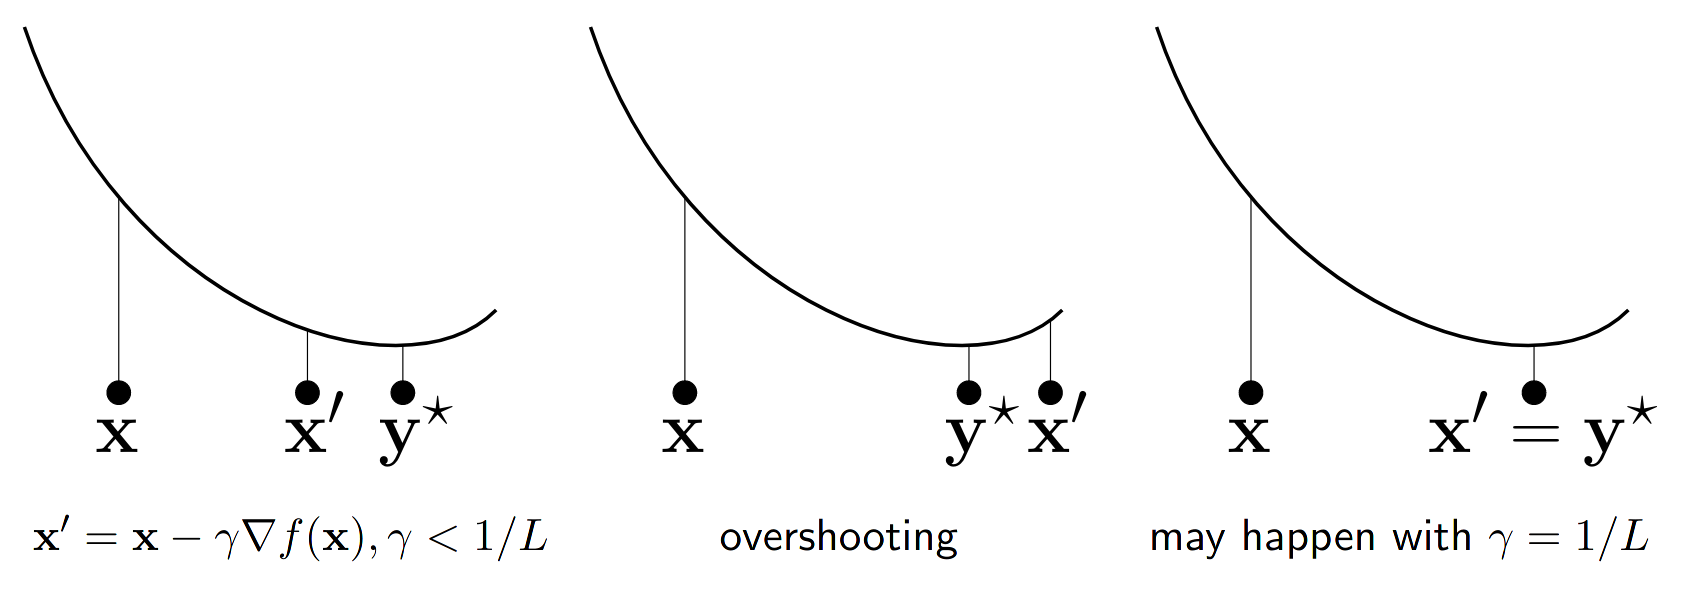
\includegraphics[width=\textwidth,height=\textheight,keepaspectratio]{no_overshooting}
  \end{figure}
\end{frame}


\section{GD for linear networks}%
\label{sec:}

\begin{frame}
  \frametitle{Trajectory Analysis}

  Even if the “landscape” (graph) of a nonconvex function has local minima, saddle
  points, and flat parts, gradient descent may avoid them and still converge to a global
  minimum.
  For this, one needs a good starting point and some theoretical understanding of what
  happens when we start there—this is trajectory analysis.

\end{frame}


\begin{frame}
  \frametitle{Linear models with several outputs}
  Recall: Learning linear models
  \begin{itemize}
    \item $n$ inputs $x_1,\dots,x_n$, where each input $x_i \in \R^d$
    \item $n$ outputs $y_1,\dots,y_n \in \R$
    \item Hypothesis (after centering):
          \begin{equation}
            y_i \approx w^T x_i ,
          \end{equation}
          for a weight vector $\bm{w} = (w_1,...,w_d) \in \R^d$ to be learned.
  \end{itemize}

  Now more than one output value:
  \begin{itemize}
    \item $n$ outputs $y_1,...,y_n$, where each output $y_i \in \R^m$
    \item Hypothesis:
          \begin{equation}
            y_i \approx W x_i,
          \end{equation}
          for a weight matrix $W \in \R{m\times d}$ to be learned.
  \end{itemize}
\end{frame}

\end{document}
